% Presentación de PULSO, versión 2 (formato de exposición, 36 diapositivas).
% El detalle de cada diapositiva está en el guion (docs/latex/guion).
% Compilar desde docs/latex/presentacion_v2:
%   latexmk -lualatex presentacion_v2.tex
\documentclass[aspectratio=169,10pt]{beamer}
\usetheme[progressbar=frametitle,numbering=fraction,block=fill,sectionpage=progressbar]{metropolis}
\usepackage{fontspec}
\usepackage[spanish,es-noshorthands,es-nodecimaldot]{babel}
\usepackage{amsmath,amssymb}
\usepackage{booktabs}
\usepackage{tikz}
\usetikzlibrary{arrows.meta,positioning}
\setmonofont{DejaVu Sans Mono}[Scale=0.78]
\graphicspath{{../figuras/}{../../../figures/}}

\definecolor{azul}{HTML}{2563A8}
\definecolor{rojo}{HTML}{C2362B}
\definecolor{verde}{HTML}{2F7D5B}
\definecolor{gris}{HTML}{5F6B77}
\setbeamercolor{frametitle}{bg=azul}
\setbeamercolor{progress bar}{fg=rojo}
\setbeamercolor{alerted text}{fg=rojo}
\setbeamercolor{block title}{bg=azul!15,fg=black}
\setbeamercolor{block body}{bg=azul!5}
\setbeamercolor{block title alerted}{bg=rojo!15,fg=black}
\setbeamercolor{block body alerted}{bg=rojo!5}
\setbeamercolor{block title example}{bg=verde!15,fg=black}
\setbeamercolor{block body example}{bg=verde!5}

\title{PULSO}
\subtitle{Pagos, Umbrales, Liquidez y Sincronización Operativa\\[2pt]
\footnotesize Redes complejas, sincronización y riesgo en sistemas de pagos digitales}
\author{Juan Diego Martínez Ayala \\ \small Dirección: Jhon Hernán Díaz Forero}
\institute{\small Semillero de Modelamiento de Sistemas Complejos y Física Computacional}
\date{Noviembre de 2026 · software v3.1.0}

\tikzset{
  c/.style={draw=#1,fill=#1!7,rounded corners=3pt,align=center,
    minimum width=11.5cm,minimum height=0.8cm,font=\small},
  etapa/.style={draw=#1,fill=#1!6,rounded corners=3pt,align=center,
    minimum width=2.6cm,minimum height=1.0cm,font=\small},
  f/.style={-{Stealth[length=2.5mm]},thick,gris}}

\begin{document}
\maketitle

\begin{frame}{Contenido}
\begin{columns}[T]
\column{0.48\textwidth}
\begin{enumerate}
\item Planteamiento
\item Modelo unificado
\item Tareas 1 a 4: de la red a las cascadas
\item Tarea 5: predicción sobre simulaciones
\end{enumerate}
\column{0.48\textwidth}
\begin{enumerate}\setcounter{enumi}{4}
\item Tarea 6: riesgo crediticio multicapa
\item Resultados
\item Implementación
\item Conclusiones
\end{enumerate}
\end{columns}
\end{frame}

% ===================================================================
\section{Planteamiento}

\begin{frame}{Contexto}
\begin{columns}[T]
\column{0.56\textwidth}
\begin{itemize}
\item Salarios, facturas y cuotas se liquidan en \textbf{sistemas de pagos digitales}
(en Colombia, \textbf{Bre-B}).
\item Cada agente paga con lo que recibe de otros: los pagos forman una
\alert{red dirigida y ponderada}.
\item La inmediatez de los pagos acelera también la transmisión de los problemas de
liquidez.
\end{itemize}
\column{0.42\textwidth}
\centering
\begin{tikzpicture}[n/.style={circle,draw=azul,fill=azul!10,minimum size=7mm},
  e/.style={-{Stealth[length=2mm]},thick}]
\node[n,fill=rojo!40] (a) at (0,0) {A};
\node[n] (b) at (1.8,0.8) {B};
\node[n] (c) at (1.8,-0.8) {C};
\node[n] (d) at (3.6,0) {D};
\draw[e] (a)--(b); \draw[e] (a)--(c); \draw[e] (b)--(d); \draw[e] (c)--(d);
\node[font=\scriptsize,align=center] at (1.8,-1.75) {El impago de A afecta a B y C\\y, a través de ellos, a D};
\end{tikzpicture}
\end{columns}
\end{frame}

\begin{frame}{Ciclos de pago y desfase}
\begin{columns}[c]
\column{0.38\textwidth}
\begin{itemize}
\item Los pagos siguen \textbf{ciclos}: nómina, facturación, cuotas.
\item Si el ingreso llega \alert{desfasado} respecto a las obligaciones propias, se
requiere más colchón.
\item El desfase genera estrés aun cuando el monto recibido no cambia.
\end{itemize}
\column{0.6\textwidth}
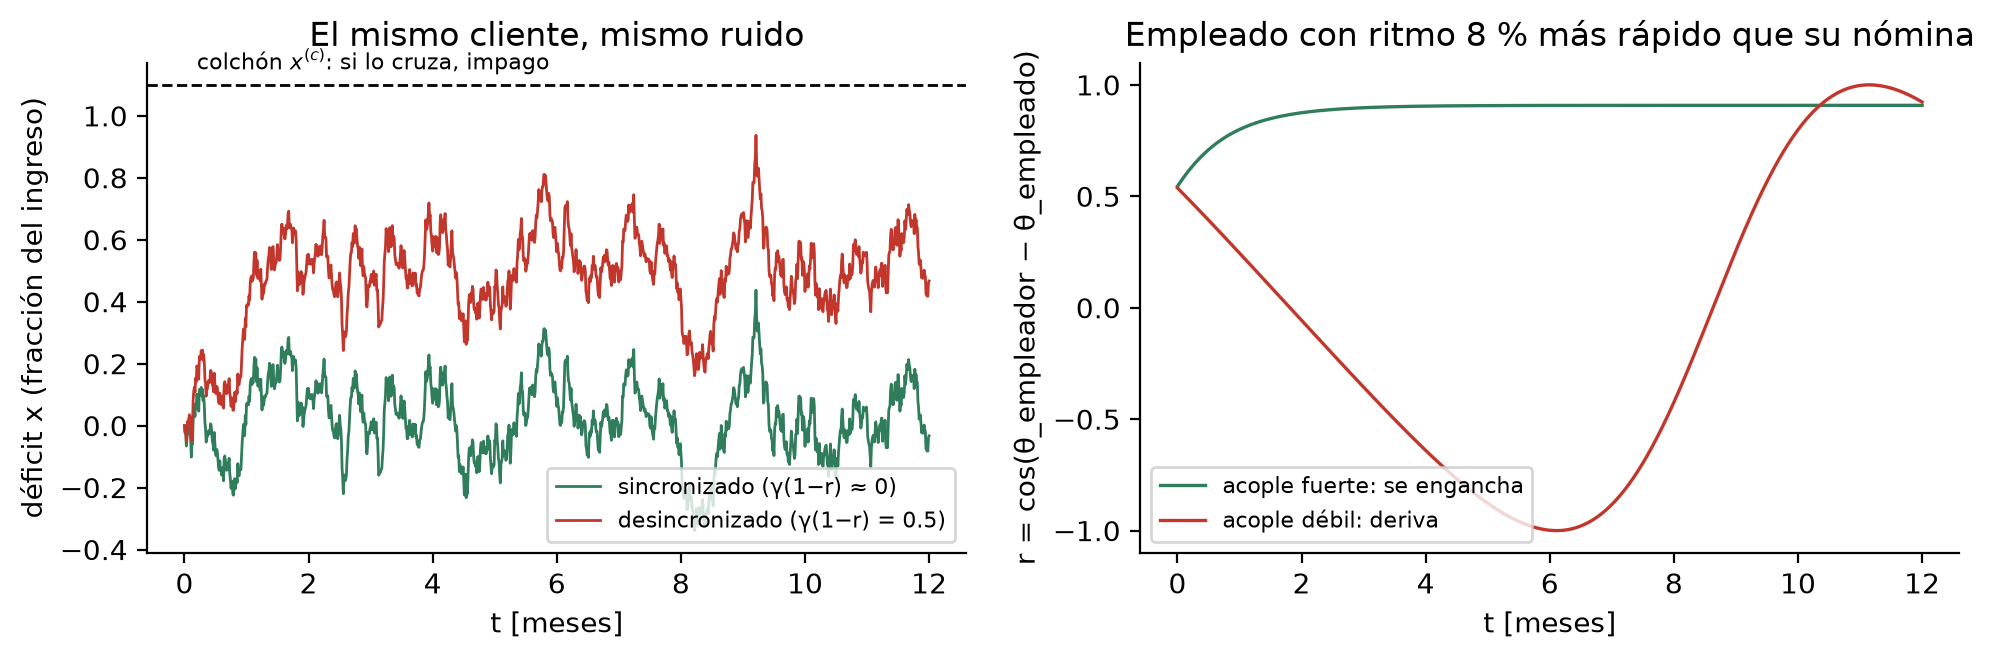
\includegraphics[width=\textwidth]{concepto_deficit_y_ritmo.png}
\end{columns}
\end{frame}

\begin{frame}{Limitación del score clásico y pregunta de investigación}
\begin{columns}[T]
\column{0.46\textwidth}
\begin{alertblock}{El score clásico no observa}
\begin{itemize}
\item la fragilidad de quienes pagan al cliente,
\item la concentración de su ingreso,
\item el desfase temporal entre ingresos y obligaciones.
\end{itemize}
\end{alertblock}
\column{0.5\textwidth}
\begin{block}{Pregunta}
¿La \textbf{sincronización} de los ciclos de pago, estimada desde las transacciones,
aporta información sobre el impago adicional a la del \textbf{score clásico} y a la de
la \textbf{red estática}?
\end{block}
\end{columns}
\end{frame}

\begin{frame}{Hipótesis y objetivos}
\begin{exampleblock}{Hipótesis falsable}
Si el ingreso desfasado genera déficit, las variables de sincronización mejoran la
predicción del impago; si ese mecanismo no existe (control nulo), no la mejoran.
\end{exampleblock}
\small
\begin{tabular}{lp{0.8\textwidth}}
\toprule
Tarea & Objetivo \\
\midrule
1 & Red de pagos y déficit nodal \\
2 & Difusión, estabilidad y recuperación \\
3 & Sincronización de los ciclos (Kuramoto) \\
4 & Umbrales de impago y cascadas \\
5 & Predicción de eventos críticos con aprendizaje automático \\
6 & Riesgo crediticio en una cartera bancaria multicapa \\
\bottomrule
\end{tabular}
\end{frame}

% ===================================================================
\section{Modelo unificado}

\begin{frame}{Un modelo, seis tareas}
\[
\frac{dx_i}{dt} = \underbrace{-\alpha x_i}_{\text{T1}}
+ \underbrace{\beta\sum_j W_{ij}x_j}_{\text{T1}}
\underbrace{- D_0(Lx)_i}_{\text{T2}}
+ \underbrace{\gamma\,k_i(1-r_i)}_{\text{T3}} + \eta_i(t)
\]
\[
\frac{d\theta_i}{dt} = \omega_i + \underbrace{\frac{K}{\langle k\rangle}\sum_j W_{ij}\sin(\theta_j-\theta_i)}_{\text{T3}},
\qquad \underbrace{x_i > x_i^{(c)} \Rightarrow \text{impago}}_{\text{T4}}
\]
\begin{itemize}
\item Déficit $x_i$ y fase del ciclo $\theta_i$ de cada entidad; $W_{ij}$: pago de $j$ a
$i$.
\item Cada tarea agrega un término; con los términos nuevos en cero se recupera
\textbf{exactamente} la tarea anterior.
\end{itemize}
\end{frame}

% ===================================================================
\section{Tareas 1 a 4: de la red a las cascadas}

\begin{frame}{Tarea 1: red de pagos e índice de amplificación}
\begin{columns}[c]
\column{0.42\textwidth}
\begin{itemize}
\item Topologías: Erdős–Rényi, Barabási–Albert y núcleo-periferia; montos lognormales.
\item Dinámica lineal $\dot x=(-\alpha I+\beta W)x$.
\item Estabilidad:
\[\boxed{R=\frac{\beta\,\rho(W)}{\alpha}<1}\]
\item Vectores propios: importancia y vulnerabilidad de cada entidad.
\end{itemize}
\column{0.56\textwidth}
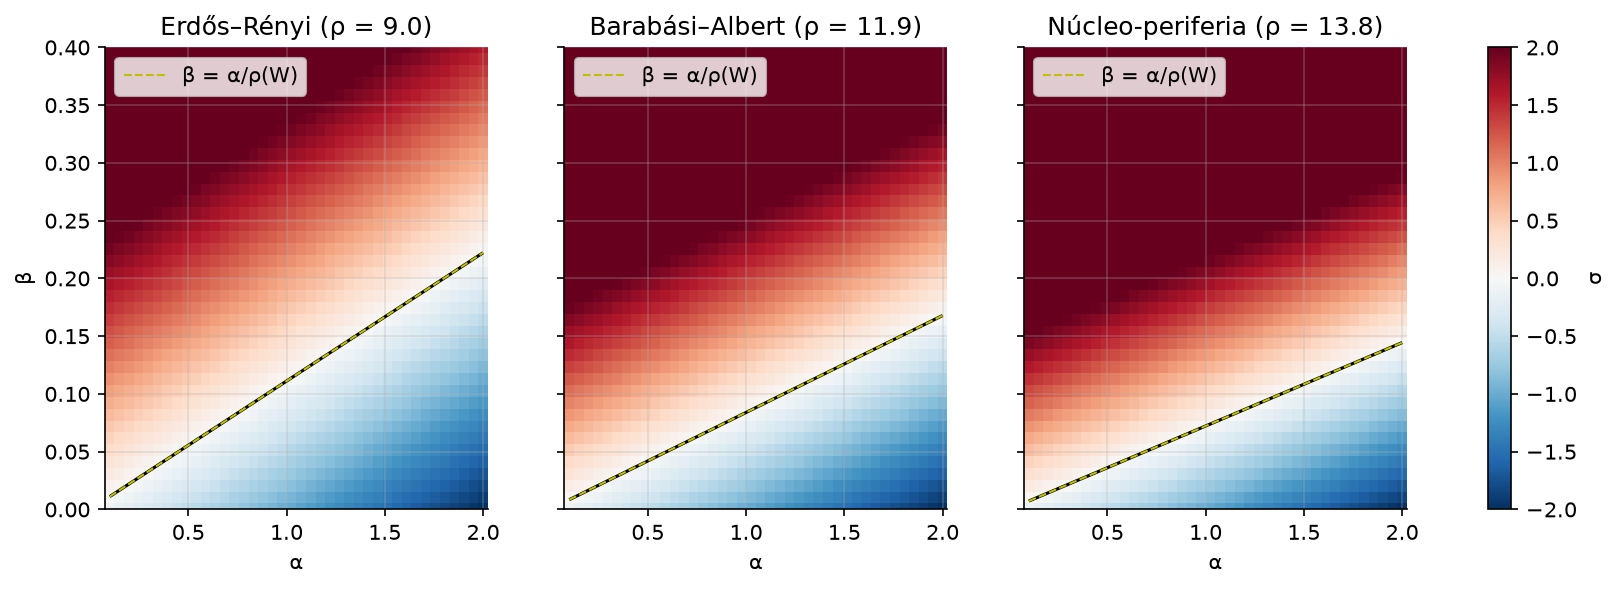
\includegraphics[width=\textwidth]{fase1_diagrama_alpha_beta.png}
\end{columns}
\end{frame}

\begin{frame}{Tarea 2: redistribución y estabilidad}
\begin{columns}[c]
\column{0.38\textwidth}
\small
\begin{itemize}
\item Laplaciano de flujo $L=D_\text{out}-W$: traslada déficit sin crearlo
(conservación verificada a $10^{-10}$).
\item Estabilidad $\sigma=\max\mathrm{Re}\,\lambda(M)$ y recuperación
$\tau_\text{rec}=-1/\sigma$.
\item Conectividad $\lambda_2$ y comunidades por corte normalizado.
\end{itemize}
\column{0.6\textwidth}
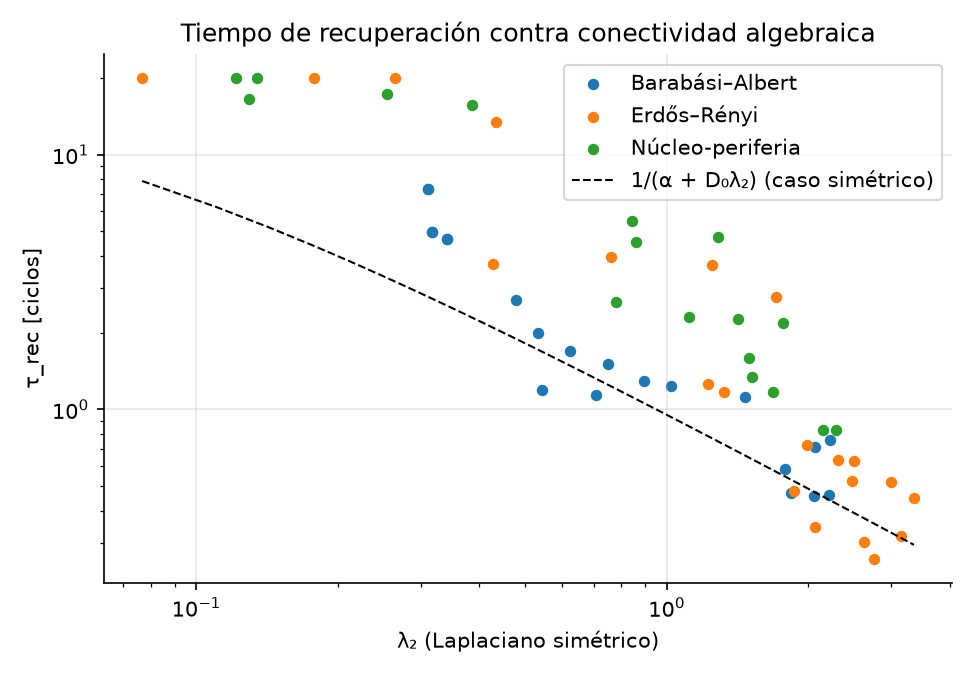
\includegraphics[width=0.49\textwidth]{fase2_tau_vs_lambda2.png}\hfill
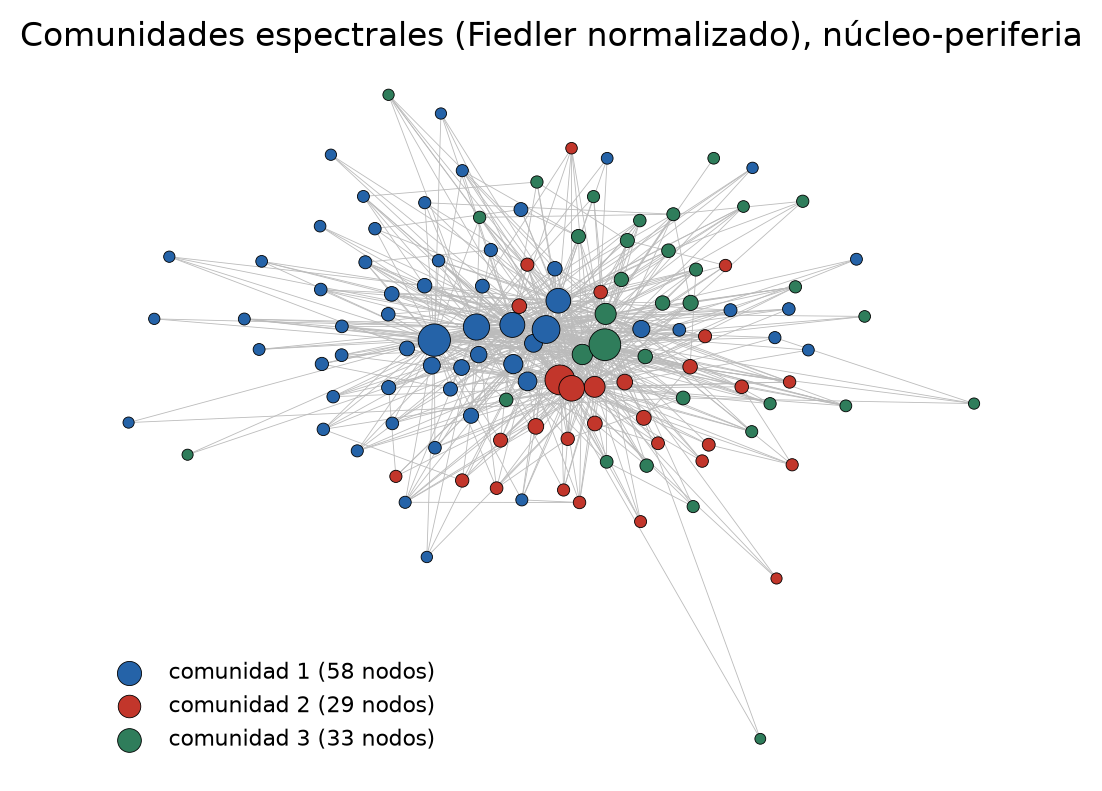
\includegraphics[width=0.49\textwidth]{fase2_comunidades_normalizado.png}
\end{columns}
\end{frame}

\begin{frame}{Tarea 3: sincronización de los ciclos de pago}
\begin{columns}[c]
\column{0.46\textwidth}
\small
\begin{itemize}
\item Modelo de Kuramoto sobre la red de pagos.
\item Coherencia local
\[r_i=\frac1{k_i}\sum_jW_{ij}\cos(\theta_j-\theta_i)\]
\item Acople al déficit: $\gamma k_i(1-r_i)$, el ingreso desfasado se vuelve déficit.
\item Red completa: $r=\sqrt{1-2\Delta/K}$ (0.7076 simulado, 0.7071 teórico).
\end{itemize}
\column{0.52\textwidth}
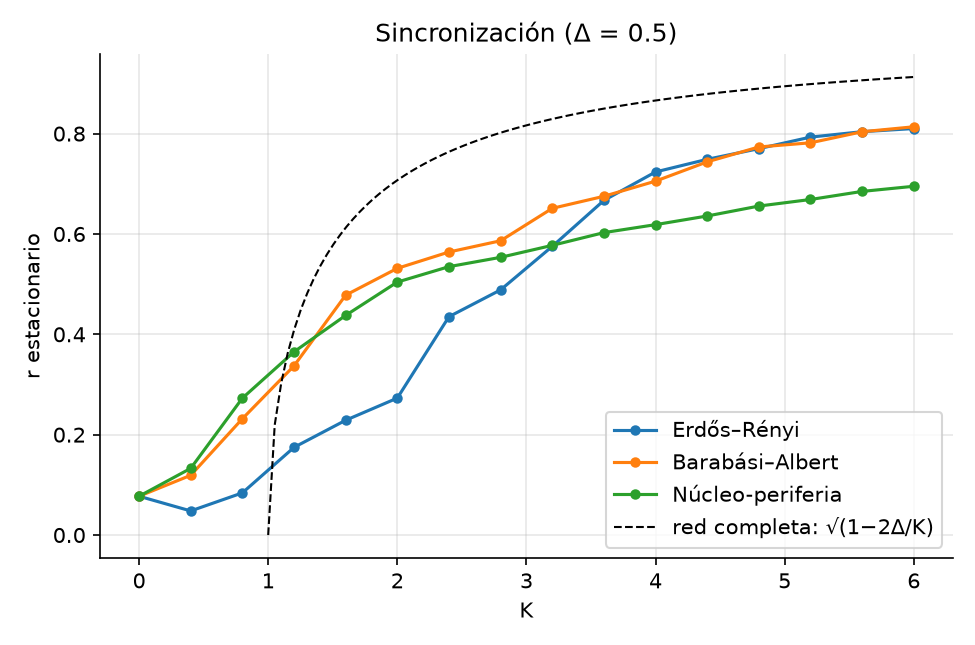
\includegraphics[width=\textwidth]{fase3_r_vs_K.png}
\end{columns}
\end{frame}

\begin{frame}{Tarea 4: impagos y cascadas}
\begin{columns}[c]
\column{0.44\textwidth}
\small
\begin{itemize}
\item Umbral $x_i^{(c)}=c\,\mathrm{out}_i\,\varepsilon_i$: al cruzarlo la entidad deja
de pagar y sus receptores pierden ingreso.
\item Choques: retiro de liquidez y caída operativa.
\item Comparación con Eisenberg–Noe, DebtRank y Watts.
\item \textbf{Ventana de contagio}: las cascadas son máximas con conectividad
intermedia.
\end{itemize}
\column{0.54\textwidth}
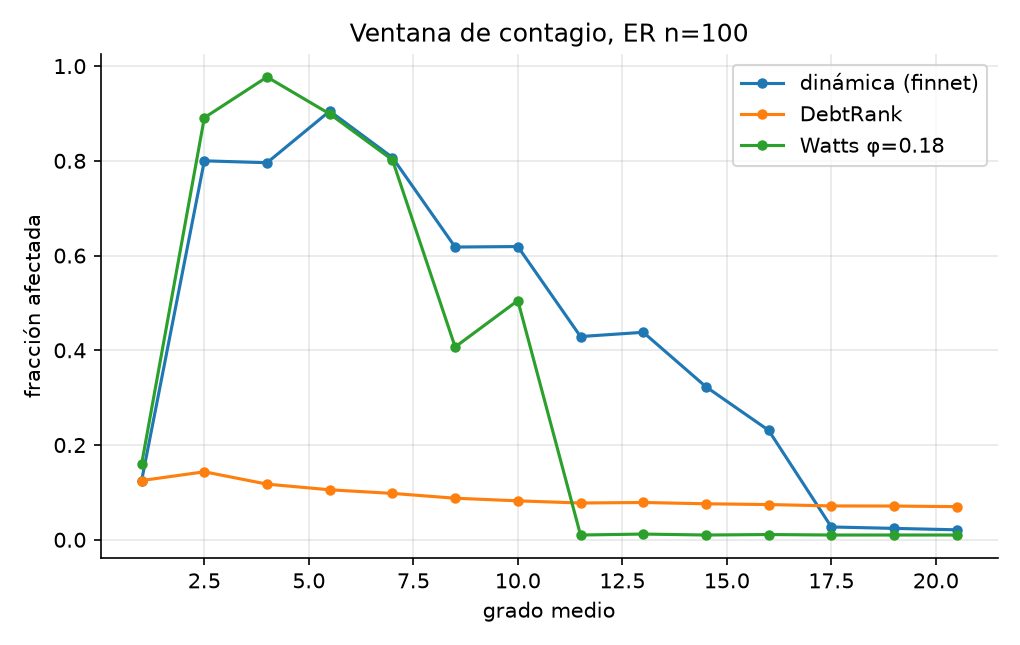
\includegraphics[width=\textwidth]{fase4_ventana_contagio.png}
\end{columns}
\end{frame}

% ===================================================================
\section{Tarea 5: predicción sobre simulaciones}

\begin{frame}{Diseño del experimento numérico}
\begin{columns}[T]
\column{0.55\textwidth}
\begin{itemize}
\item \textbf{300 redes} y \textbf{20\,000 escenarios} por hipercubo latino en 13
parámetros.
\item Muestreo concentrado cerca de $R=1$.
\item Tablas: escenarios (colapso global) y nodos (cascada por entidad).
\item Validación \textbf{GroupKFold por red}: ninguna red en entrenamiento y prueba a la
vez.
\end{itemize}
\column{0.4\textwidth}
\footnotesize
\begin{tabular}{ll}
\toprule
Parámetro & Rango \\
\midrule
$\alpha$ & $[0.5,2]$ \\
$R$ & $[0.4,1.6]$ \\
$K$ & $[0,6]$ \\
$\gamma$ & $[0,0.08]$ \\
colchón $c$ & $[0.2,1.5]$ \\
pérdida $\lambda$ & $[0.3,1.5]$ \\
\bottomrule
\end{tabular}
\end{columns}
\end{frame}

\begin{frame}{Tarea 5: resultados}
\begin{columns}[c]
\column{0.48\textwidth}
\footnotesize
\begin{tabular}{lll}
\toprule
Modelo & Objetivo & Desempeño \\
\midrule
Logística & colapso & AUC 0.957 \\
XGBoost & colapso & AUC \textbf{0.980} \\
XGBoost & cascada & $R^2$ 0.50 \\
GCN & cascada & $R^2$ \textbf{0.60} \\
\bottomrule
\end{tabular}
\vspace{0.3cm}

\small
\begin{itemize}
\item Predicción en milisegundos frente a segundos de simulación.
\item PINN: recupera $\gamma$ y $K$ con error $<1~\%$.
\end{itemize}
\column{0.5\textwidth}
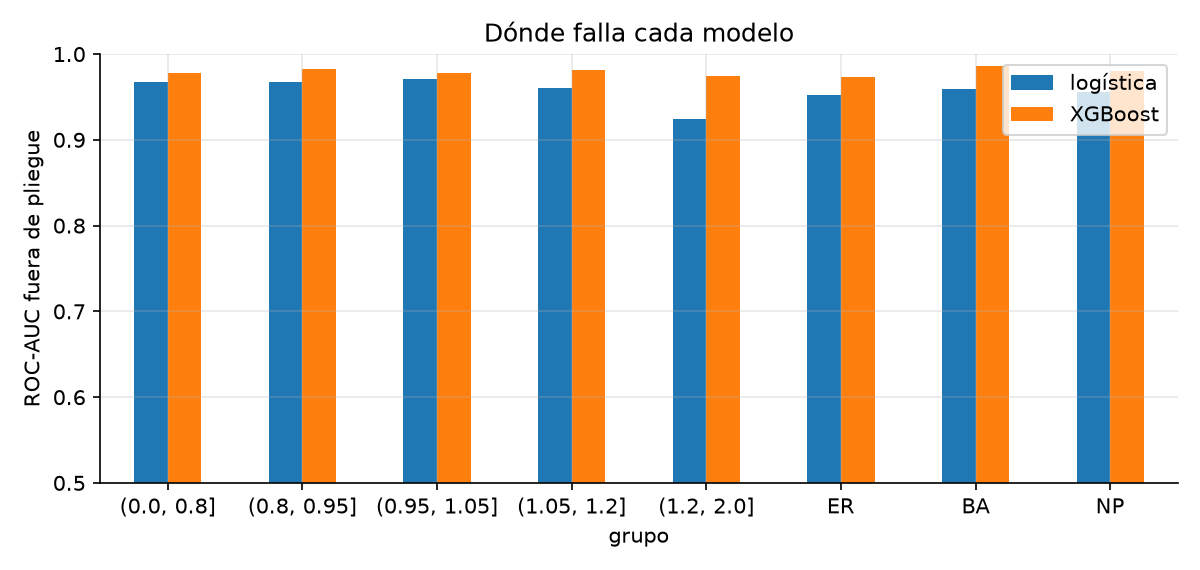
\includegraphics[width=\textwidth]{fase6_comparacion_modelos.png}
\end{columns}
\end{frame}

% ===================================================================
\section{Tarea 6: riesgo crediticio multicapa}

\begin{frame}{De entidades a clientes de un banco}
\begin{columns}[T]
\column{0.42\textwidth}
\begin{itemize}
\item Nodos: \textbf{personas} y \textbf{firmas} clientes de un banco.
\item No hay datos públicos de esta red: se \textbf{genera} una cartera con un mecanismo
conocido y se verifica que el método lo recupera.
\item El banco solo observa atributos y el \textbf{registro de transacciones}.
\end{itemize}
\column{0.56\textwidth}
\footnotesize
\begin{tabular}{llll}
\toprule
Capa & Dirección & Ciclo & Contagio \\
\midrule
N · nómina & F $\to$ P & 15/30 días & fuerte \\
S · proveedores & F $\to$ F & facturas & moderado \\
T · transferencias & P $\to$ P & irregular & débil \\
\bottomrule
\end{tabular}
\end{columns}
\end{frame}

\begin{frame}{Cartera sintética}
\begin{columns}[c]
\column{0.5\textwidth}
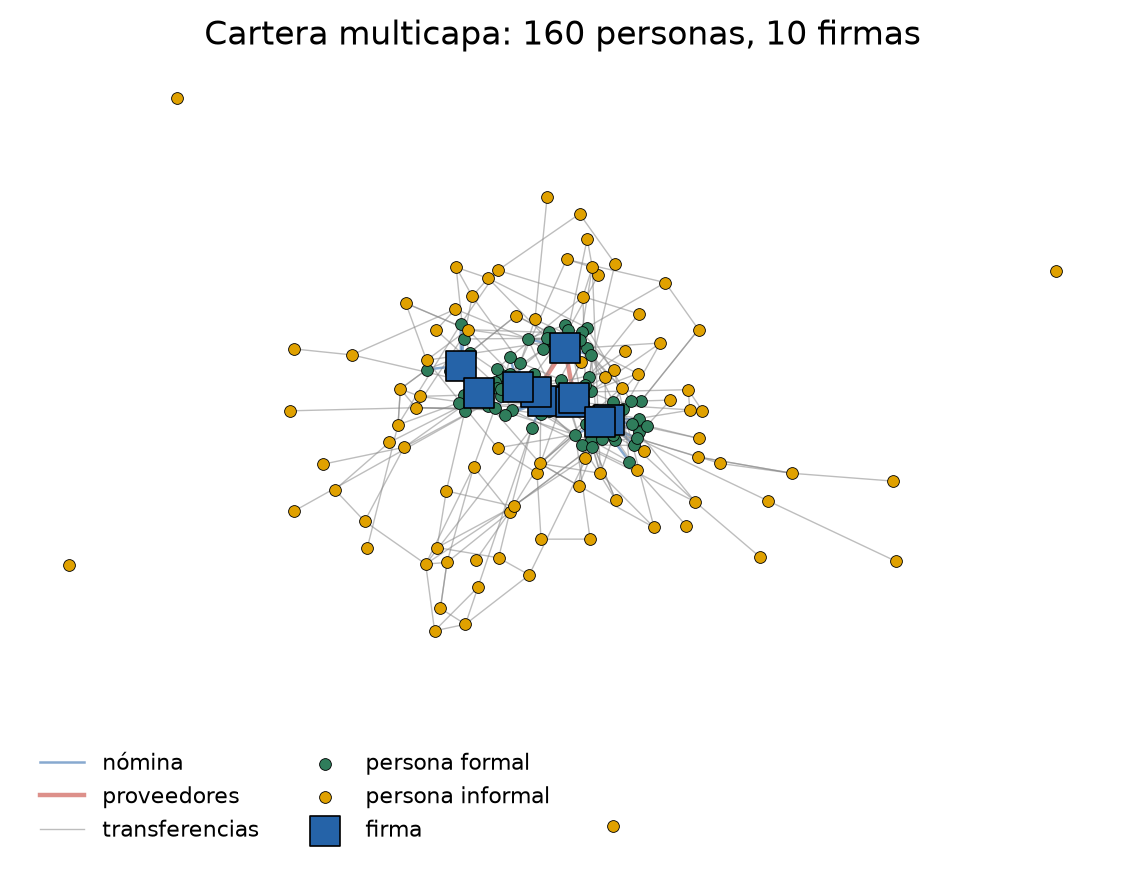
\includegraphics[width=\textwidth]{tarea6_red_multicapa.png}
\scriptsize Ejemplo reducido (160 personas, 10 firmas) para visualizar las capas.
\column{0.48\textwidth}
\small
\begin{itemize}
\item 2000 personas y 100 firmas; 55~\% de informalidad.
\item Firmas de tamaño Pareto; nómina mensual o quincenal.
\item Formales: ritmo heredado del empleador. Informales: ritmos dispersos.
\item PD verdadera logística en variables clásicas más un componente latente;
columnas \texttt{truth\_*} vetadas para los modelos.
\end{itemize}
\end{columns}
\end{frame}

\begin{frame}{Modelo dinámico multicapa}
\[
\dot x_i = -\alpha x_i + \sum_\ell\beta_\ell\sum_j\frac{W^\ell_{ij}}{s_i}x_j
+ \gamma\frac{k_i}{s_i}(1-r_i) + \sigma\xi_i(t)
\]
\[
\dot\theta_i = \omega_i + \sum_\ell K_\ell\sum_j\frac{W^\ell_{ij}}{k_i}\sin(\theta_j-\theta_i),
\qquad x_i^{(c)} = c\Bigl(\frac{\mathrm{PD}_\text{ref}}{\mathrm{PD}_i}\Bigr)^{\kappa}\varepsilon_i
\]
\begin{itemize}
\item Tiempo en meses; déficit como fracción del ingreso total $s_i$.
\item Contagio y acople \textbf{por capa}; impagos idiosincráticos según la PD.
\item Con una capa se recupera el modelo de las tareas 1–4.
\end{itemize}
\end{frame}

\begin{frame}{Del modelo a lo que observa el banco}
\begin{columns}[c]
\column{0.5\textwidth}
\small
\begin{itemize}
\item Cada ciclo completo de un pagador genera sus pagos y su cuota al banco: tabla
\texttt{(t, src, dst, layer, amount)}.
\item Observación: meses 0–6. Predicción: meses 6–18.
\item Estimación: $\hat W$, fase por eventos $\hat\theta$ y coherencia $\hat r_i(t)$.
\item Error mediano $<5~\%$ en $\hat W$; correlación $\hat r$–$r>0.8$.
\end{itemize}
\column{0.48\textwidth}
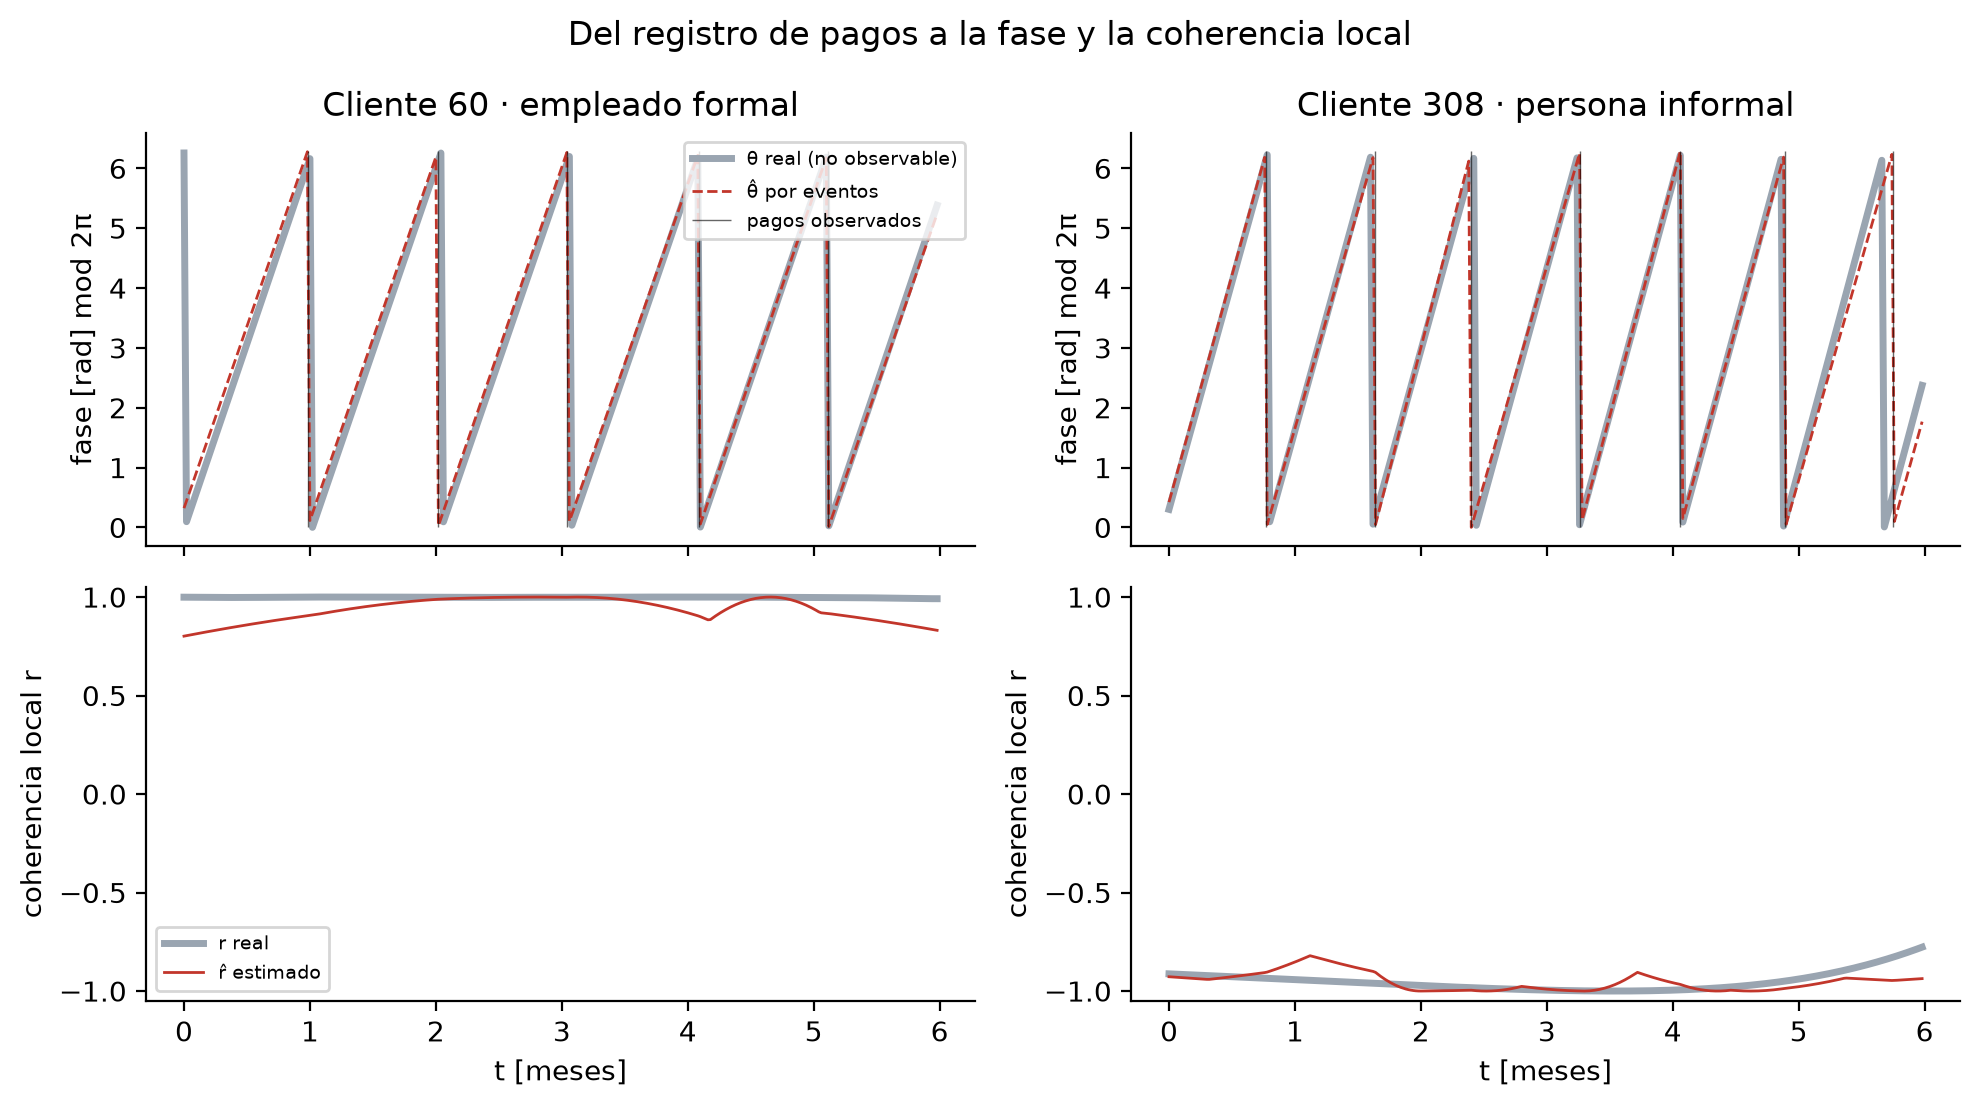
\includegraphics[width=\textwidth]{tarea6_fase_eventos.png}
\end{columns}
\end{frame}

\begin{frame}{Variables en tres niveles y protocolo}
\footnotesize
\begin{tabular}{p{0.17\textwidth}p{0.77\textwidth}}
\toprule
Nivel & Variables \\
\midrule
1 · Clásico & ingreso, endeudamiento, edad, antigüedad, productos, moras, formalidad \\
2 · Red estática & composición y concentración del ingreso, PageRank, salud del
empleador y de los pagadores \\
3 · Red dinámica & coherencia $\hat r$ y su variabilidad, desfase, desajuste de
ritmo, irregularidad de ciclos, pagadores que cesaron \\
\bottomrule
\end{tabular}
\vspace{0.3cm}

\small
\begin{columns}[T]
\column{0.48\textwidth}
\textbf{Regímenes}: con red y \textbf{nulo} ($\beta_\ell=\gamma=\lambda=0$, mismos
sorteos).
\column{0.48\textwidth}
\textbf{Evaluación}: 20 carteras por régimen, GroupKFold por cartera, diferencias
pareadas con IC 95~\%.
\end{columns}
\end{frame}

% ===================================================================
\section{Resultados}

\begin{frame}{Validación numérica}
\begin{columns}[T]
\column{0.48\textwidth}
\footnotesize
\begin{tabular}{ll}
\toprule
Verificación & Resultado \\
\midrule
RK4 frente a $e^{Mt}x_0$ & error $<10^{-6}$ \\
Conservación bajo difusión & $<10^{-10}$ \\
Kuramoto, red completa & 0.7076 / 0.7071 \\
Una capa frente a v1 & idénticos \\
$\hat r_i$ frente a $r_i$ & corr.\ $>0.8$ \\
Dataset regenerado & idéntico bit a bit \\
\bottomrule
\end{tabular}
\column{0.48\textwidth}
\vspace{0.6cm}
\centering
\Large\textbf{127} pruebas automáticas superadas

\vspace{0.3cm}
\small unitarias, analíticas, de integración y de interfaz
\end{columns}
\end{frame}

\begin{frame}{Carteras simuladas}
\begin{columns}[c]
\column{0.46\textwidth}
\small
\begin{tabular}{lcc}
\toprule
 & Nulo & Con red \\
\midrule
Clientes & 40\,404 & 37\,431 \\
Impago a 12 meses & 5.9~\% & 9.6~\% \\
$R$ & 0 & 0.09–0.17 \\
\bottomrule
\end{tabular}
\vspace{0.3cm}

Formales sincronizados con su nómina; informales con $\hat r\approx0$.
\column{0.52\textwidth}
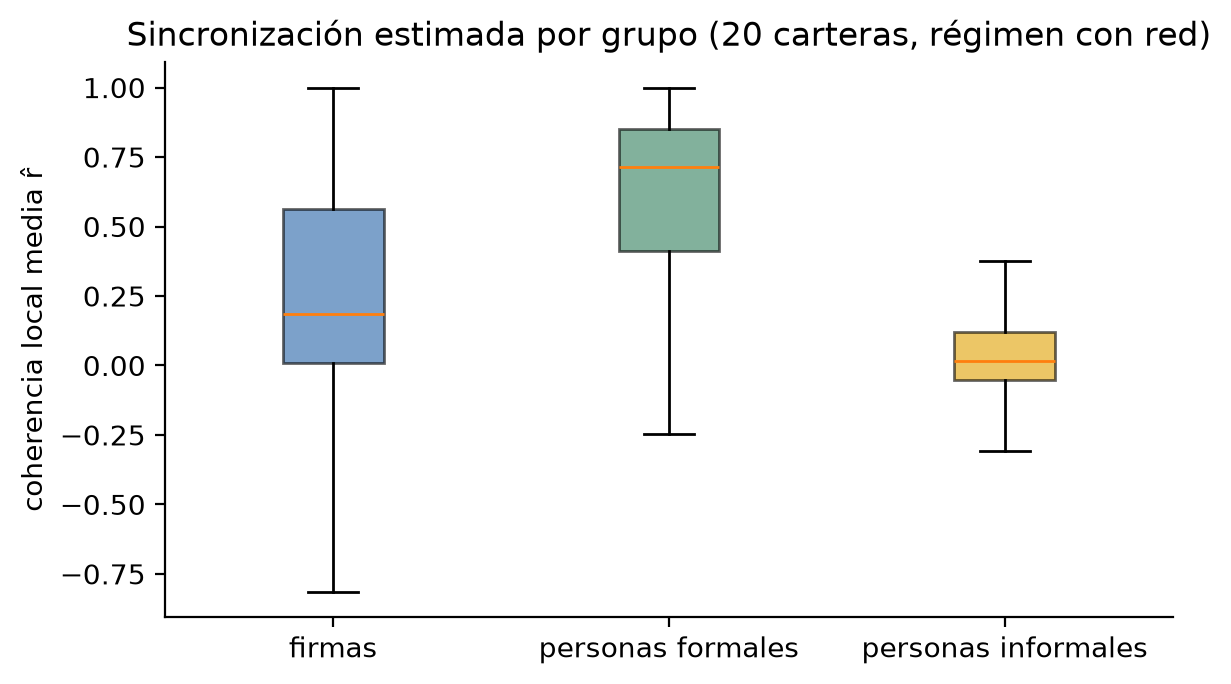
\includegraphics[width=\textwidth]{tarea6_sincronia_grupos.png}
\end{columns}
\end{frame}

\begin{frame}{Desempeño predictivo por nivel}
\centering
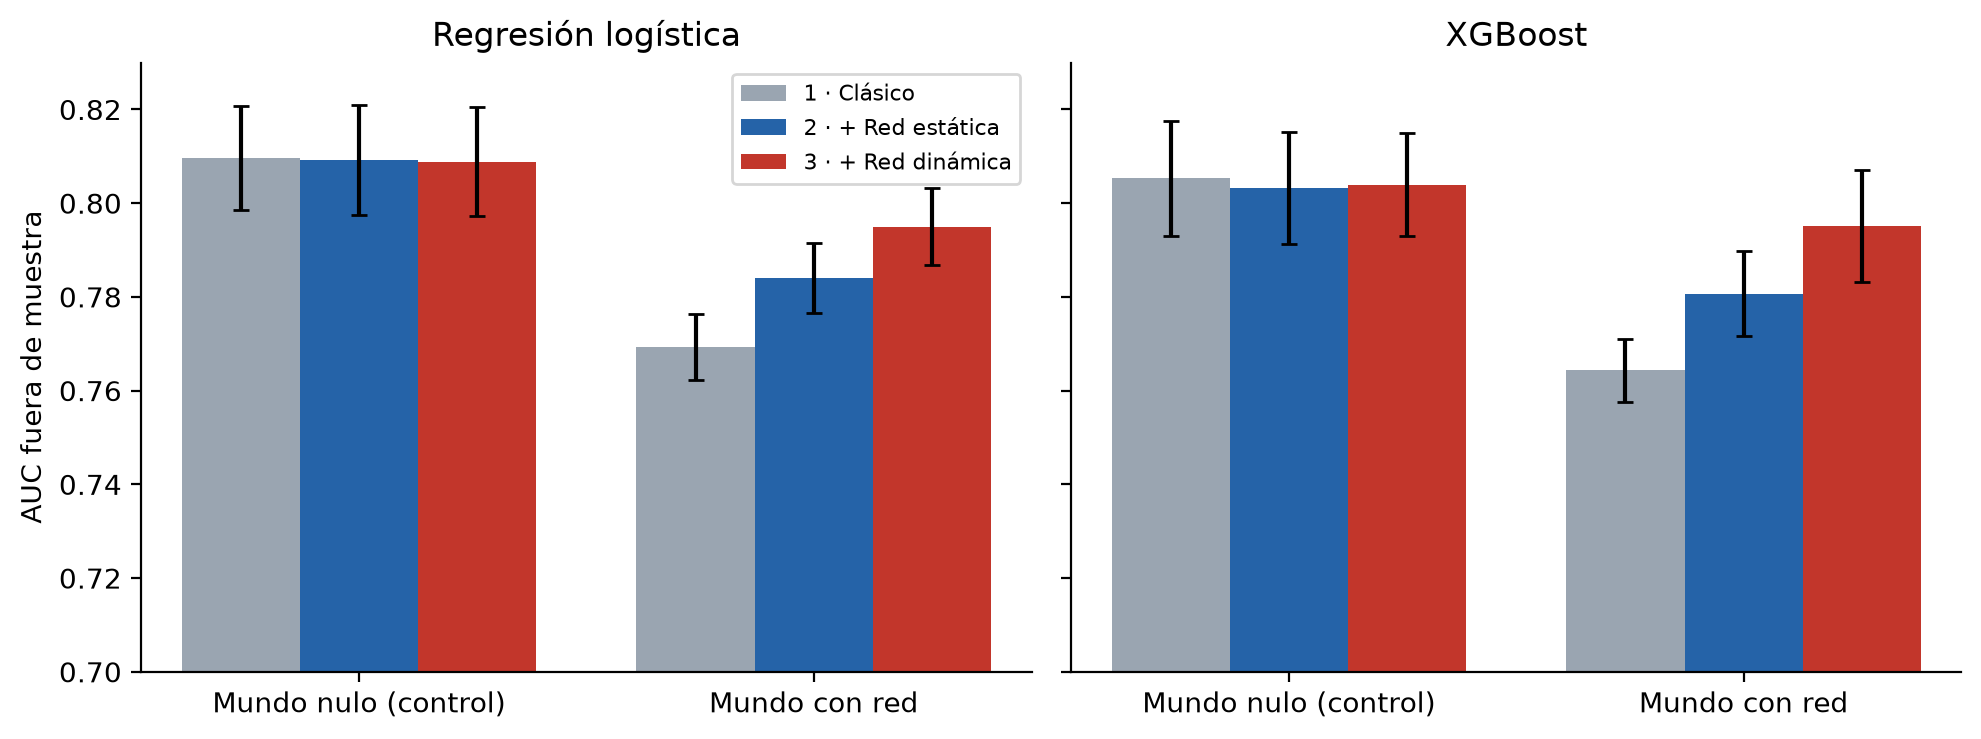
\includegraphics[width=0.6\textwidth]{tarea6_auc_niveles.png}

\footnotesize
\begin{tabular}{lcccc}
\toprule
Régimen con red & AUC log. & AUC XGB & PR-AUC log. & KS log. \\
\midrule
1 · Clásico & 0.769 & 0.764 & 0.277 & 0.416 \\
2 · + Estática & 0.784 & 0.781 & 0.307 & 0.437 \\
3 · + Dinámica & \textbf{0.795} & \textbf{0.795} & \textbf{0.323} & \textbf{0.457} \\
\bottomrule
\end{tabular}
\end{frame}

\begin{frame}{Mejoras pareadas y control nulo}
\begin{columns}[c]
\column{0.6\textwidth}
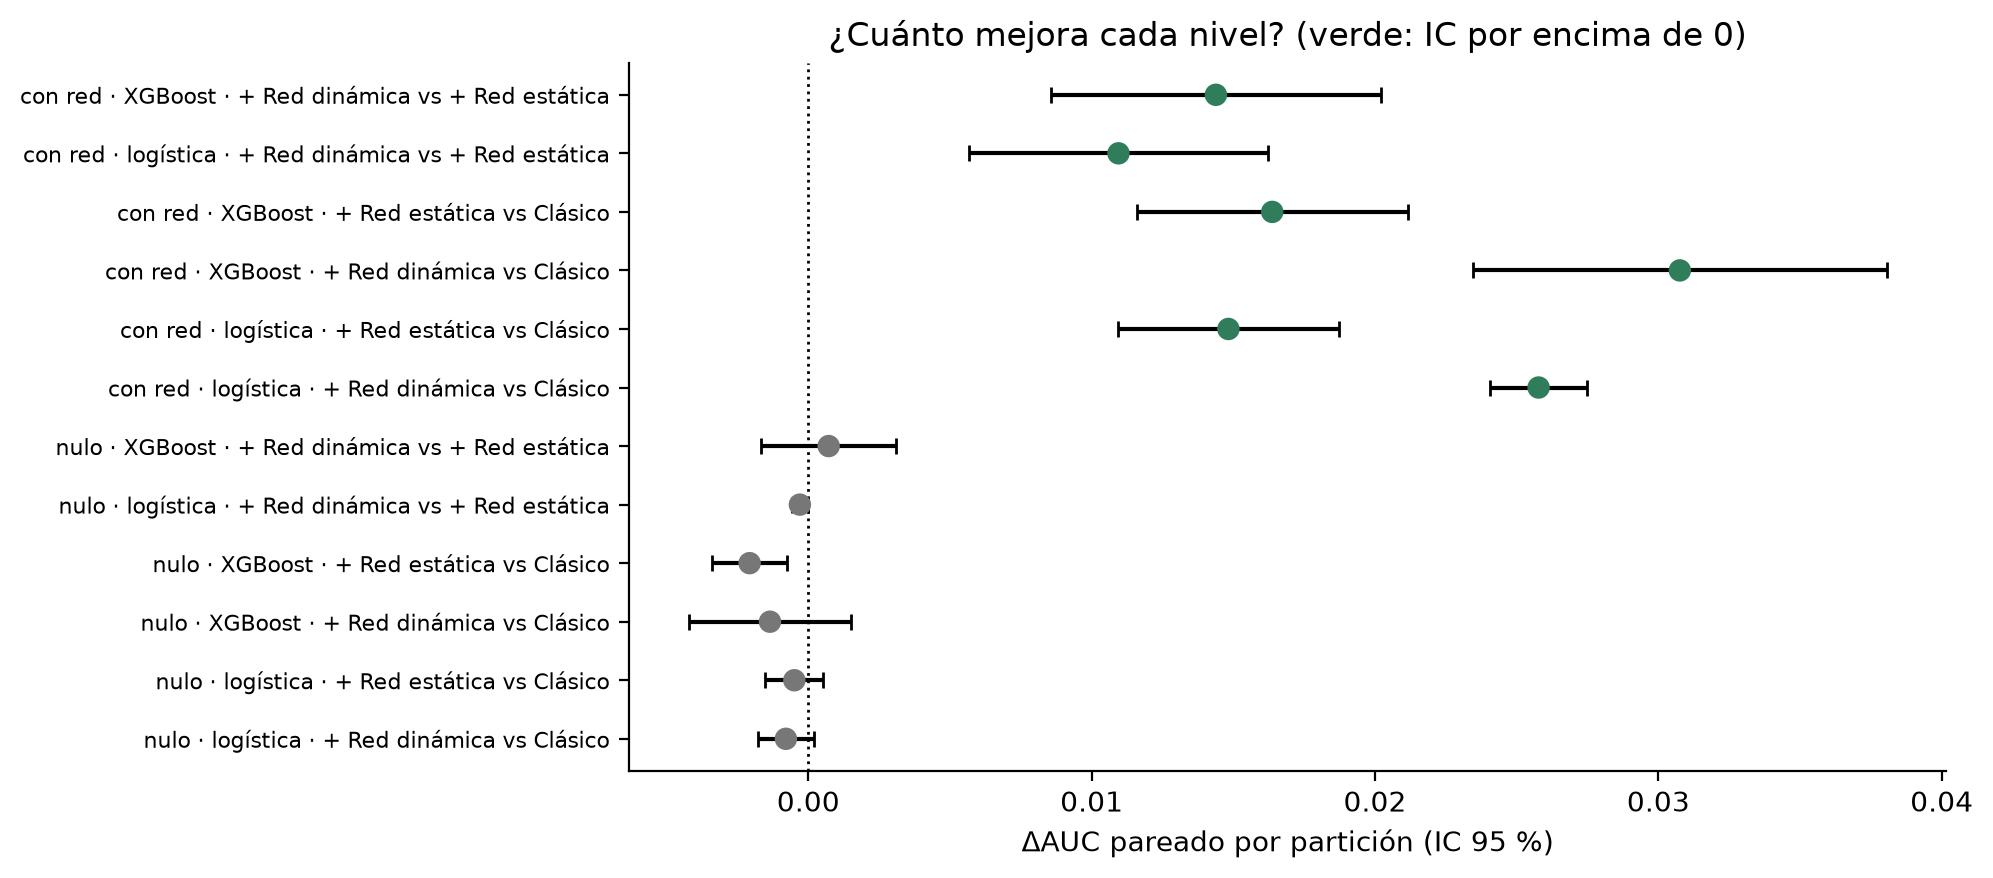
\includegraphics[width=\textwidth]{tarea6_mejoras.png}
\column{0.38\textwidth}
\begin{exampleblock}{Con red: dinámica vs.\ estática}
\small $\Delta\mathrm{AUC}=+0.011$ $[+0.006,+0.016]$ (logística)\\
$+0.014$ $[+0.009,+0.020]$ (XGBoost)\\
positiva en 5 de 5 particiones
\end{exampleblock}
\begin{alertblock}{Nulo}
\small $\Delta\mathrm{AUC}\in[-0.002,+0.001]$: sin fuga de información.
\end{alertblock}
\end{columns}
\end{frame}

\begin{frame}{Respuesta a la intensidad del mecanismo}
\begin{columns}[c]
\column{0.56\textwidth}
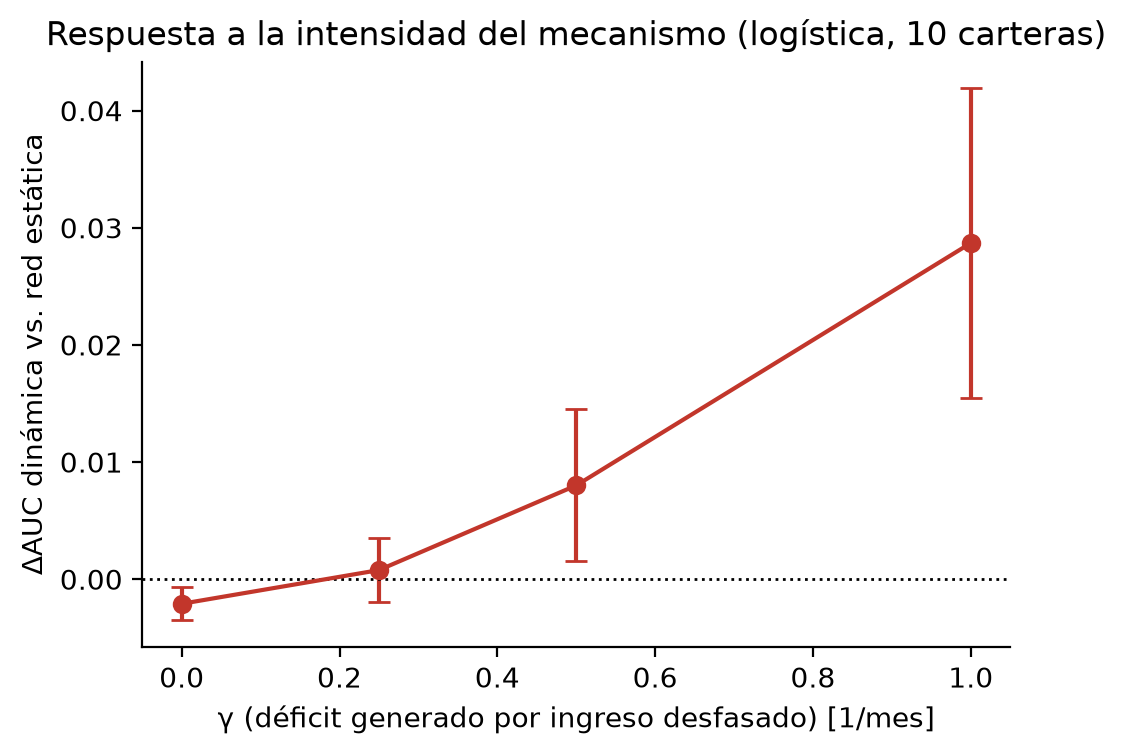
\includegraphics[width=\textwidth]{tarea6_sensibilidad_gamma.png}
\column{0.42\textwidth}
\begin{center}
\small
\begin{tabular}{cc}
\toprule
$\gamma$ [1/mes] & $\Delta\mathrm{AUC}$ \\
\midrule
0 & $-0.002$ \\
0.25 & $+0.001$ \\
0.5 & $+0.008$ \\
1.0 & $+0.029$ \\
\bottomrule
\end{tabular}
\end{center}
\small La ganancia proviene de la \textbf{desincronización}, no del contagio, y crece de
forma monótona con $\gamma$.
\end{columns}
\end{frame}

\begin{frame}{Interpretación y relación sincronía--impago}
\begin{columns}[c]
\column{0.5\textwidth}
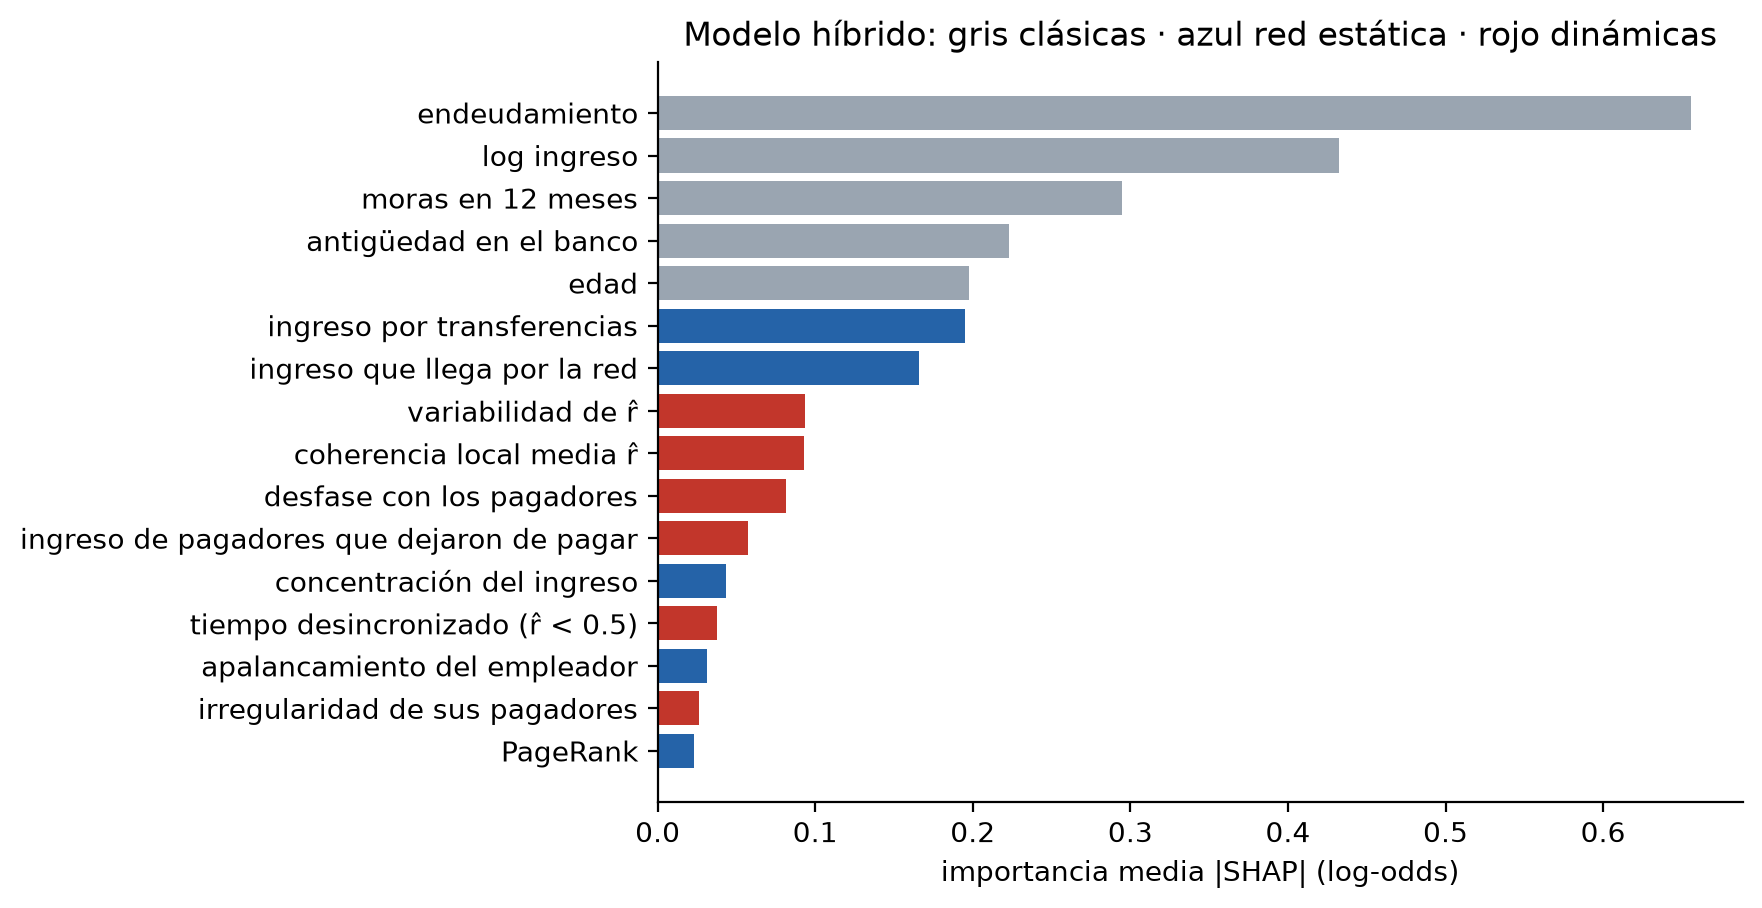
\includegraphics[width=\textwidth]{tarea6_shap.png}
\scriptsize Las variables clásicas dominan; las dinámicas aportan información adicional.
\column{0.48\textwidth}
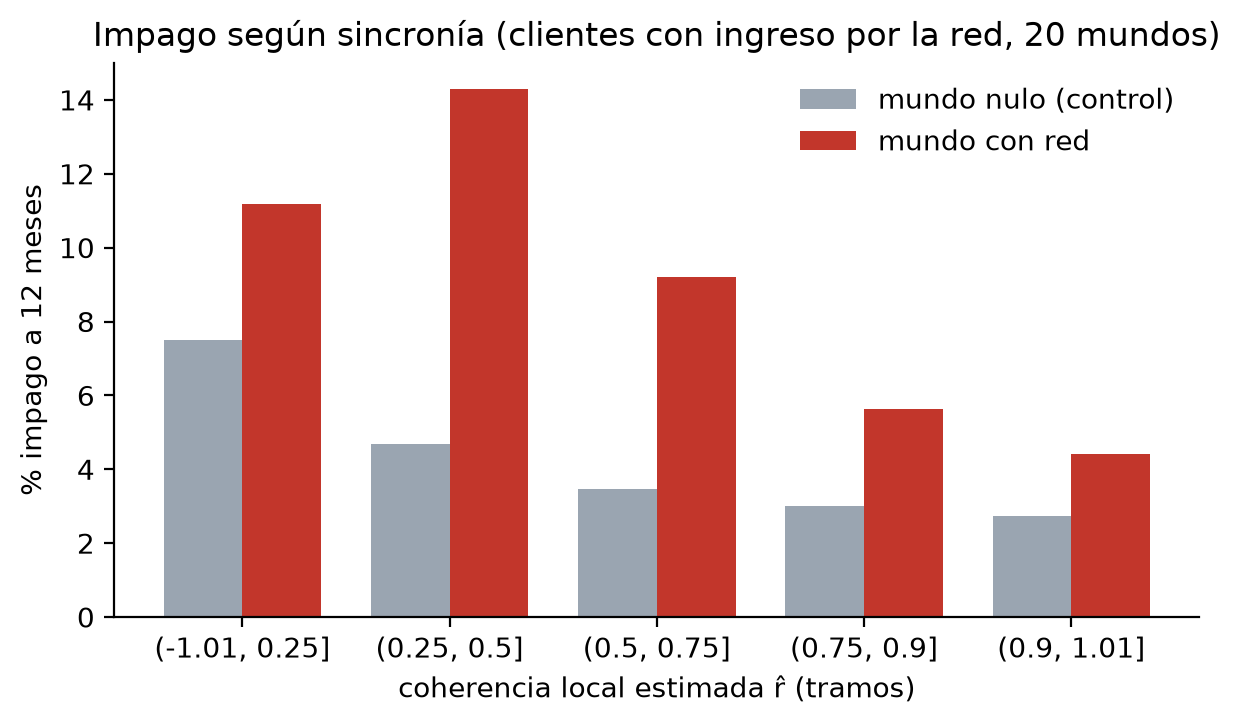
\includegraphics[width=\textwidth]{tarea6_impago_por_r.png}
\scriptsize Con red, el impago pasa de 4.4~\% ($\hat r>0.9$) a 11–14~\% ($\hat r<0.5$).
\end{columns}
\end{frame}

\begin{frame}{Escenario: quiebra de un empleador}
\begin{columns}[c]
\column{0.58\textwidth}
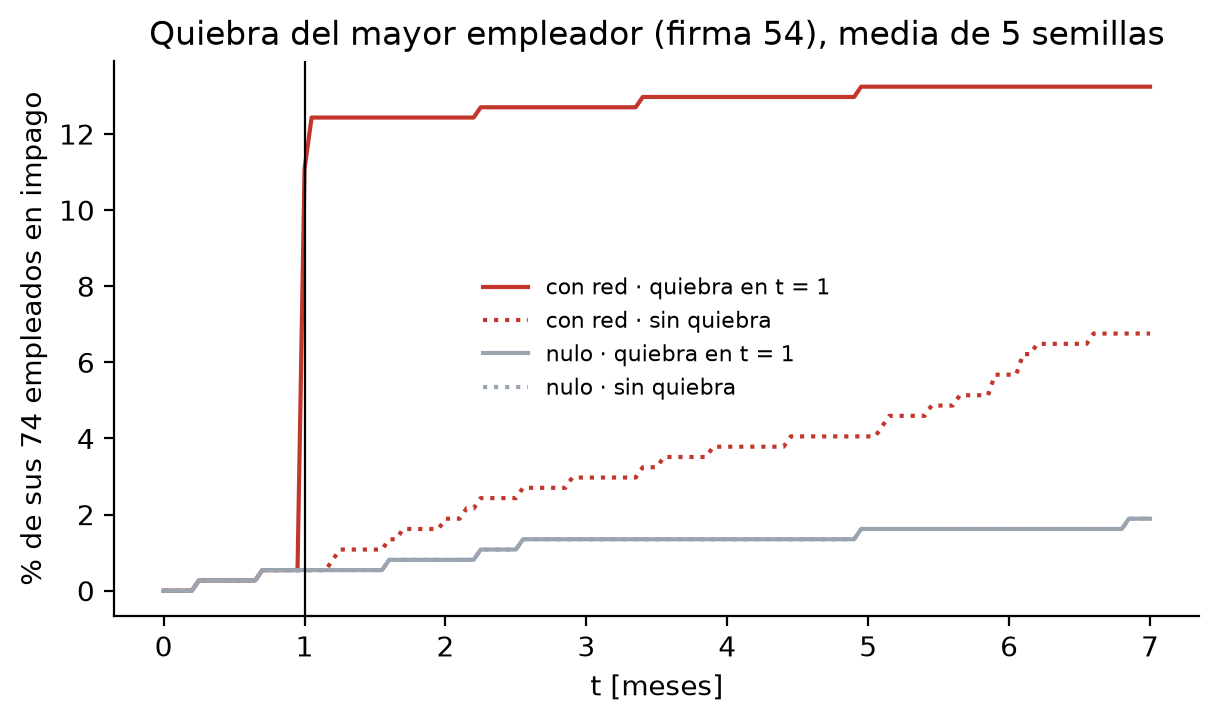
\includegraphics[width=\textwidth]{tarea6_quiebra.png}
\column{0.4\textwidth}
\small
\begin{itemize}
\item Quiebra del mayor empleador (74 empleados) en $t=1$ mes.
\item 12~\% de los empleados cae de inmediato; 13~\% a los 6 meses frente a 7~\% sin
quiebra.
\item En el régimen nulo no hay efecto.
\item Uso: pruebas de estrés por concentración en empleadores.
\end{itemize}
\end{columns}
\end{frame}

\begin{frame}{Alcance e interpretación}
\small
\begin{columns}[T]
\column{0.48\textwidth}
\begin{exampleblock}{Lo que el diseño respalda}
\begin{itemize}
\item El mecanismo, si existe, es \textbf{detectable} con transacciones.
\item La dinámica aporta información ausente en la red estática.
\item El aporte se anula sin mecanismo y crece con él.
\end{itemize}
\end{exampleblock}
\column{0.48\textwidth}
\begin{alertblock}{Limitaciones}
\begin{itemize}
\item Datos sintéticos: no prueba el mecanismo en una cartera real.
\item Parámetros ilustrativos.
\item Red completamente observable dentro del banco.
\end{itemize}
\end{alertblock}
\end{columns}
\end{frame}

% ===================================================================
\section{Implementación}

\begin{frame}{Arquitectura y reproducibilidad}
\centering
\begin{tikzpicture}
\node[c=azul] (a) {\textbf{Interfaz} · \texttt{app/} (Streamlit, 9 páginas)};
\node[c=verde,below=0.25cm of a] (b) {\textbf{Servicio} · \texttt{service.py}, \texttt{credit/service.py}};
\node[c=rojo,below=0.25cm of b] (c) {\textbf{Núcleo} · modelo, integración, espectro, cascadas, ML, \texttt{world/}, \texttt{credit/}};
\node[c=orange,below=0.25cm of c] (d) {\textbf{Configuración y datos} · \texttt{configs/*.yaml}, \texttt{data/}, \texttt{models/}};
\draw[f] (a)--(b); \draw[f] (b)--(c); \draw[f] (c)--(d);
\end{tikzpicture}

\vspace{0.3cm}
\small Parámetros en YAML · semillas explícitas · esquemas validados · 127 pruebas ·
integración continua · Docker
\end{frame}

\begin{frame}{Flujo de datos de la tarea 6}
\centering
\begin{tikzpicture}[node distance=0.45cm]
\node[etapa=azul] (w) {cartera\\sintética};
\node[etapa=azul,right=of w] (m) {modelo\\multicapa};
\node[etapa=azul,right=of m] (t) {registro de\\transacciones};
\node[etapa=azul,right=of t] (e) {estimación\\$\hat W,\hat\theta,\hat r$};
\node[etapa=azul,below=0.7cm of e] (v) {variables\\3 niveles};
\node[etapa=azul,left=of v] (cv) {GroupKFold\\por cartera};
\node[etapa=azul,left=of cv] (d) {mejoras pareadas\\control nulo};
\node[etapa=rojo,left=of d] (o) {resultados y\\modelos finales};
\draw[f] (w)--(m); \draw[f] (m)--(t); \draw[f] (t)--(e); \draw[f] (e)--(v);
\draw[f] (v)--(cv); \draw[f] (cv)--(d); \draw[f] (d)--(o);
\end{tikzpicture}

\vspace{0.4cm}
\small \texttt{uv run pulso credit configs/credit.yaml} ejecuta el flujo completo.
\end{frame}

\begin{frame}{Aplicación web}
\begin{columns}[c]
\column{0.49\textwidth}
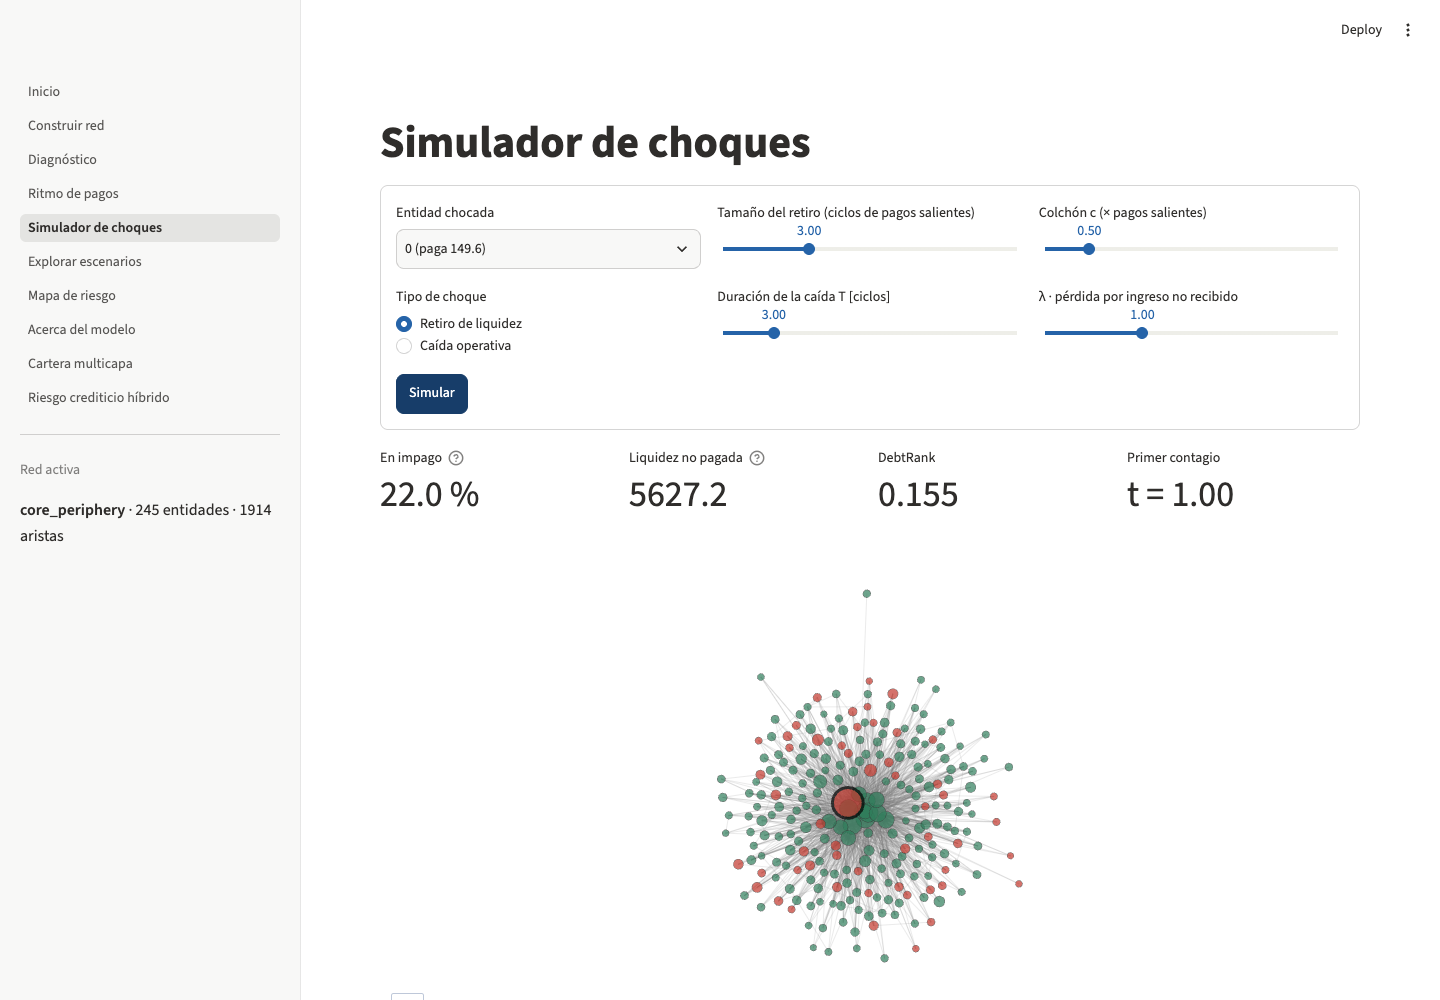
\includegraphics[width=\textwidth]{app_simulador.png}
\scriptsize Simulador de choques (tareas 1–4).
\column{0.49\textwidth}
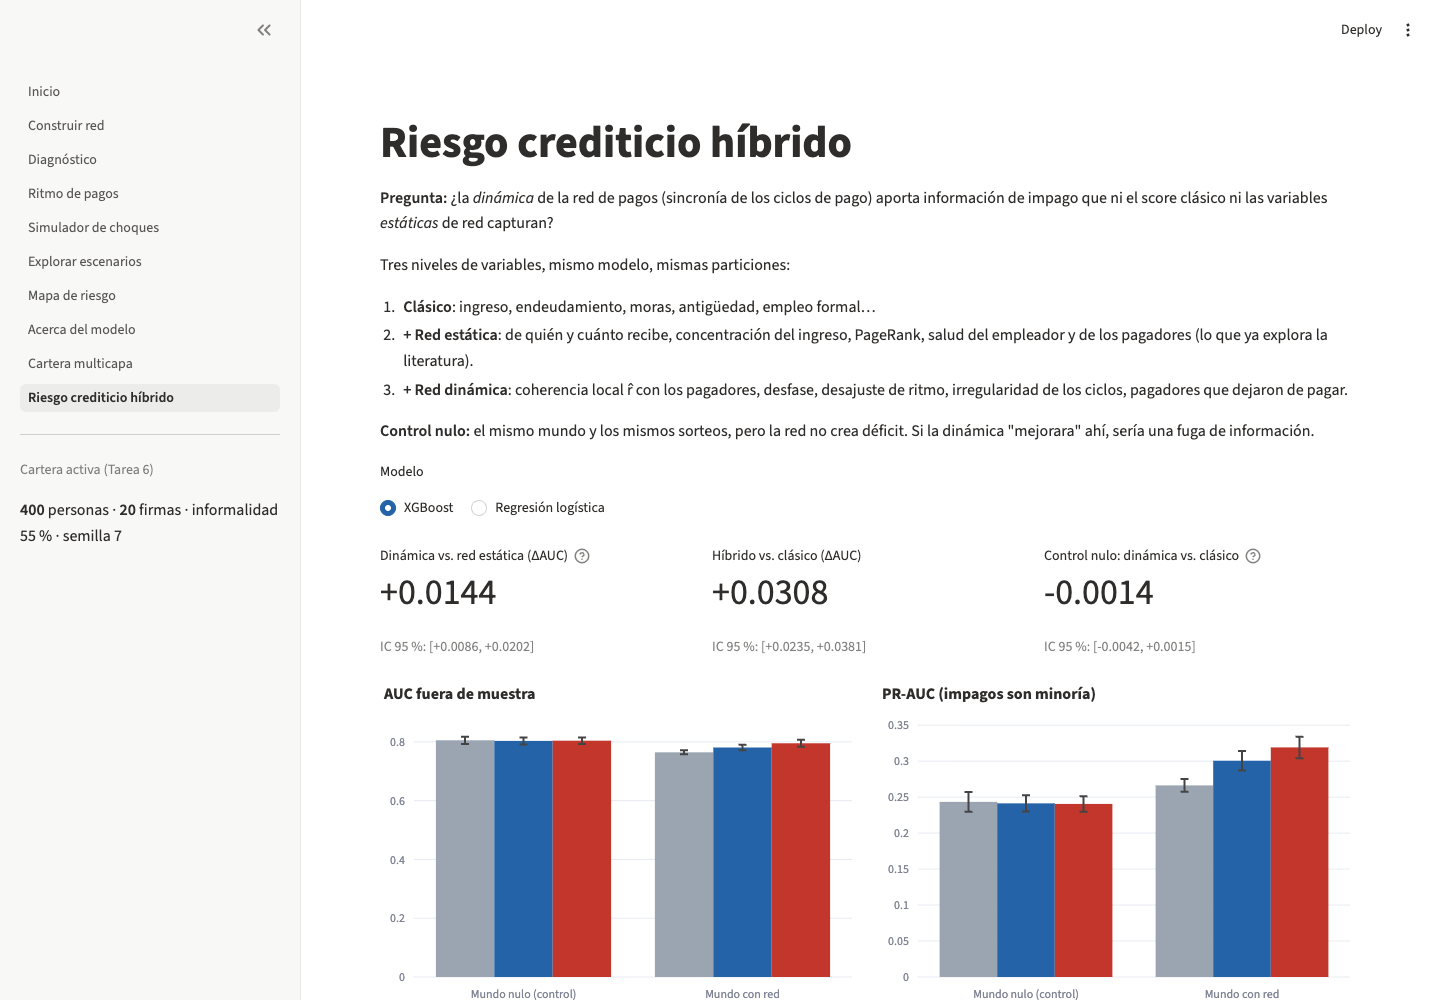
\includegraphics[width=\textwidth]{app_hibrido.png}
\scriptsize Riesgo crediticio híbrido (tarea 6).
\end{columns}
\end{frame}

% ===================================================================
\section{Conclusiones}

\begin{frame}{Conclusiones}
\begin{enumerate}
\item Un único modelo integra contagio, redistribución, sincronización y cascadas, y cada
componente se valida contra resultados analíticos.
\item $R=\beta\rho(W)/\alpha$ y el espectro del operador indican cuándo la red amortigua
o amplifica.
\item El aprendizaje automático predice el colapso con AUC 0.98 en milisegundos.
\item En una cartera multicapa, la sincronización estimada desde transacciones mejora la
predicción del impago sobre la red estática, sin efecto en el control nulo.
\item El software es reproducible, está probado y se ejecuta como aplicación web.
\end{enumerate}
\end{frame}

\begin{frame}{Trabajo futuro}
\begin{itemize}
\item \textbf{Validación empírica} con una cartera real anonimizada.
\item \textbf{Revisión sistemática} de la literatura.
\item Fecha de cuota y plazos como \textbf{forzamiento externo} del ritmo.
\item \textbf{Retroalimentación}: el déficit modifica el ritmo de pago.
\item \textbf{Observabilidad parcial}: un banco frente al operador de Bre-B.
\end{itemize}
\end{frame}

\begin{frame}{Referencias principales}
\scriptsize
\begin{columns}[T]
\column{0.5\textwidth}
\begin{itemize}
\item Acebrón et al. (2005). The Kuramoto model. \emph{Rev.\ Mod.\ Phys.}
\item Battiston et al. (2012). DebtRank. \emph{Sci.\ Rep.}
\item Boccaletti et al. (2014). Multilayer networks. \emph{Phys.\ Rep.}
\item Eisenberg y Noe (2001). \emph{Management Science}.
\item Kipf y Welling (2017). GCN. \emph{ICLR}.
\item Letizia y Lillo (2019). \emph{EPJ Data Science}.
\end{itemize}
\column{0.5\textwidth}
\begin{itemize}
\item Newman (2010). \emph{Networks}. Oxford.
\item Pikovsky, Rosenblum y Kurths (2001). \emph{Synchronization}.
\item Raissi, Perdikaris y Karniadakis (2019). PINN. \emph{J.\ Comput.\ Phys.}
\item Rodrigues et al. (2016). \emph{Phys.\ Rep.}
\item Shi y Malik (2000). \emph{IEEE TPAMI}.
\item Watts (2002). \emph{PNAS}.
\end{itemize}
\end{columns}
\end{frame}

\begin{frame}[standout]
Gracias

\vspace{0.4cm}
\normalsize Guía, guion y manual: \texttt{docs/Presentaciones/}
\end{frame}

\end{document}
